% Exploratory Data Analysis Section
% Earthquake Prediction Problems - Data Science Report

This section presents an exploratory data analysis (EDA) of the USGS earthquake dataset (2002-2025), focusing on insights relevant to magnitude prediction, depth classification, and seismic hotspot identification.

\subsection{Dataset Overview}

The dataset contains \textbf{2,921,770 earthquake records} with the following key features:

\begin{table}[H]
\centering
\begin{tabular}{|l|l|l|}
\hline
\textbf{Feature} & \textbf{Description} & \textbf{Range} \\
\hline
Latitude & Geographic coordinate & -90 to 90 \\
Longitude & Geographic coordinate & -180 to 180 \\
Depth & Earthquake depth (km) & 0 to 735.8 \\
Magnitude & Earthquake magnitude & -9.99 to 9.1 \\
nst & Number of seismic stations & 0 to 934 \\
gap & Azimuthal gap (degrees) & 6.5 to 360 \\
depth\_category & Shallow/Intermediate/Deep & 3 classes \\
\hline
\end{tabular}
\caption{Key features in the earthquake dataset}
\end{table}

%==============================================================================
\subsection{Magnitude Analysis}
%==============================================================================

\subsubsection{Magnitude Distribution}

Figure \ref{fig:magnitude_dist} shows the distribution of earthquake magnitudes, which is fundamental for understanding earthquake occurrence patterns.

\begin{figure}[H]
    \centering
    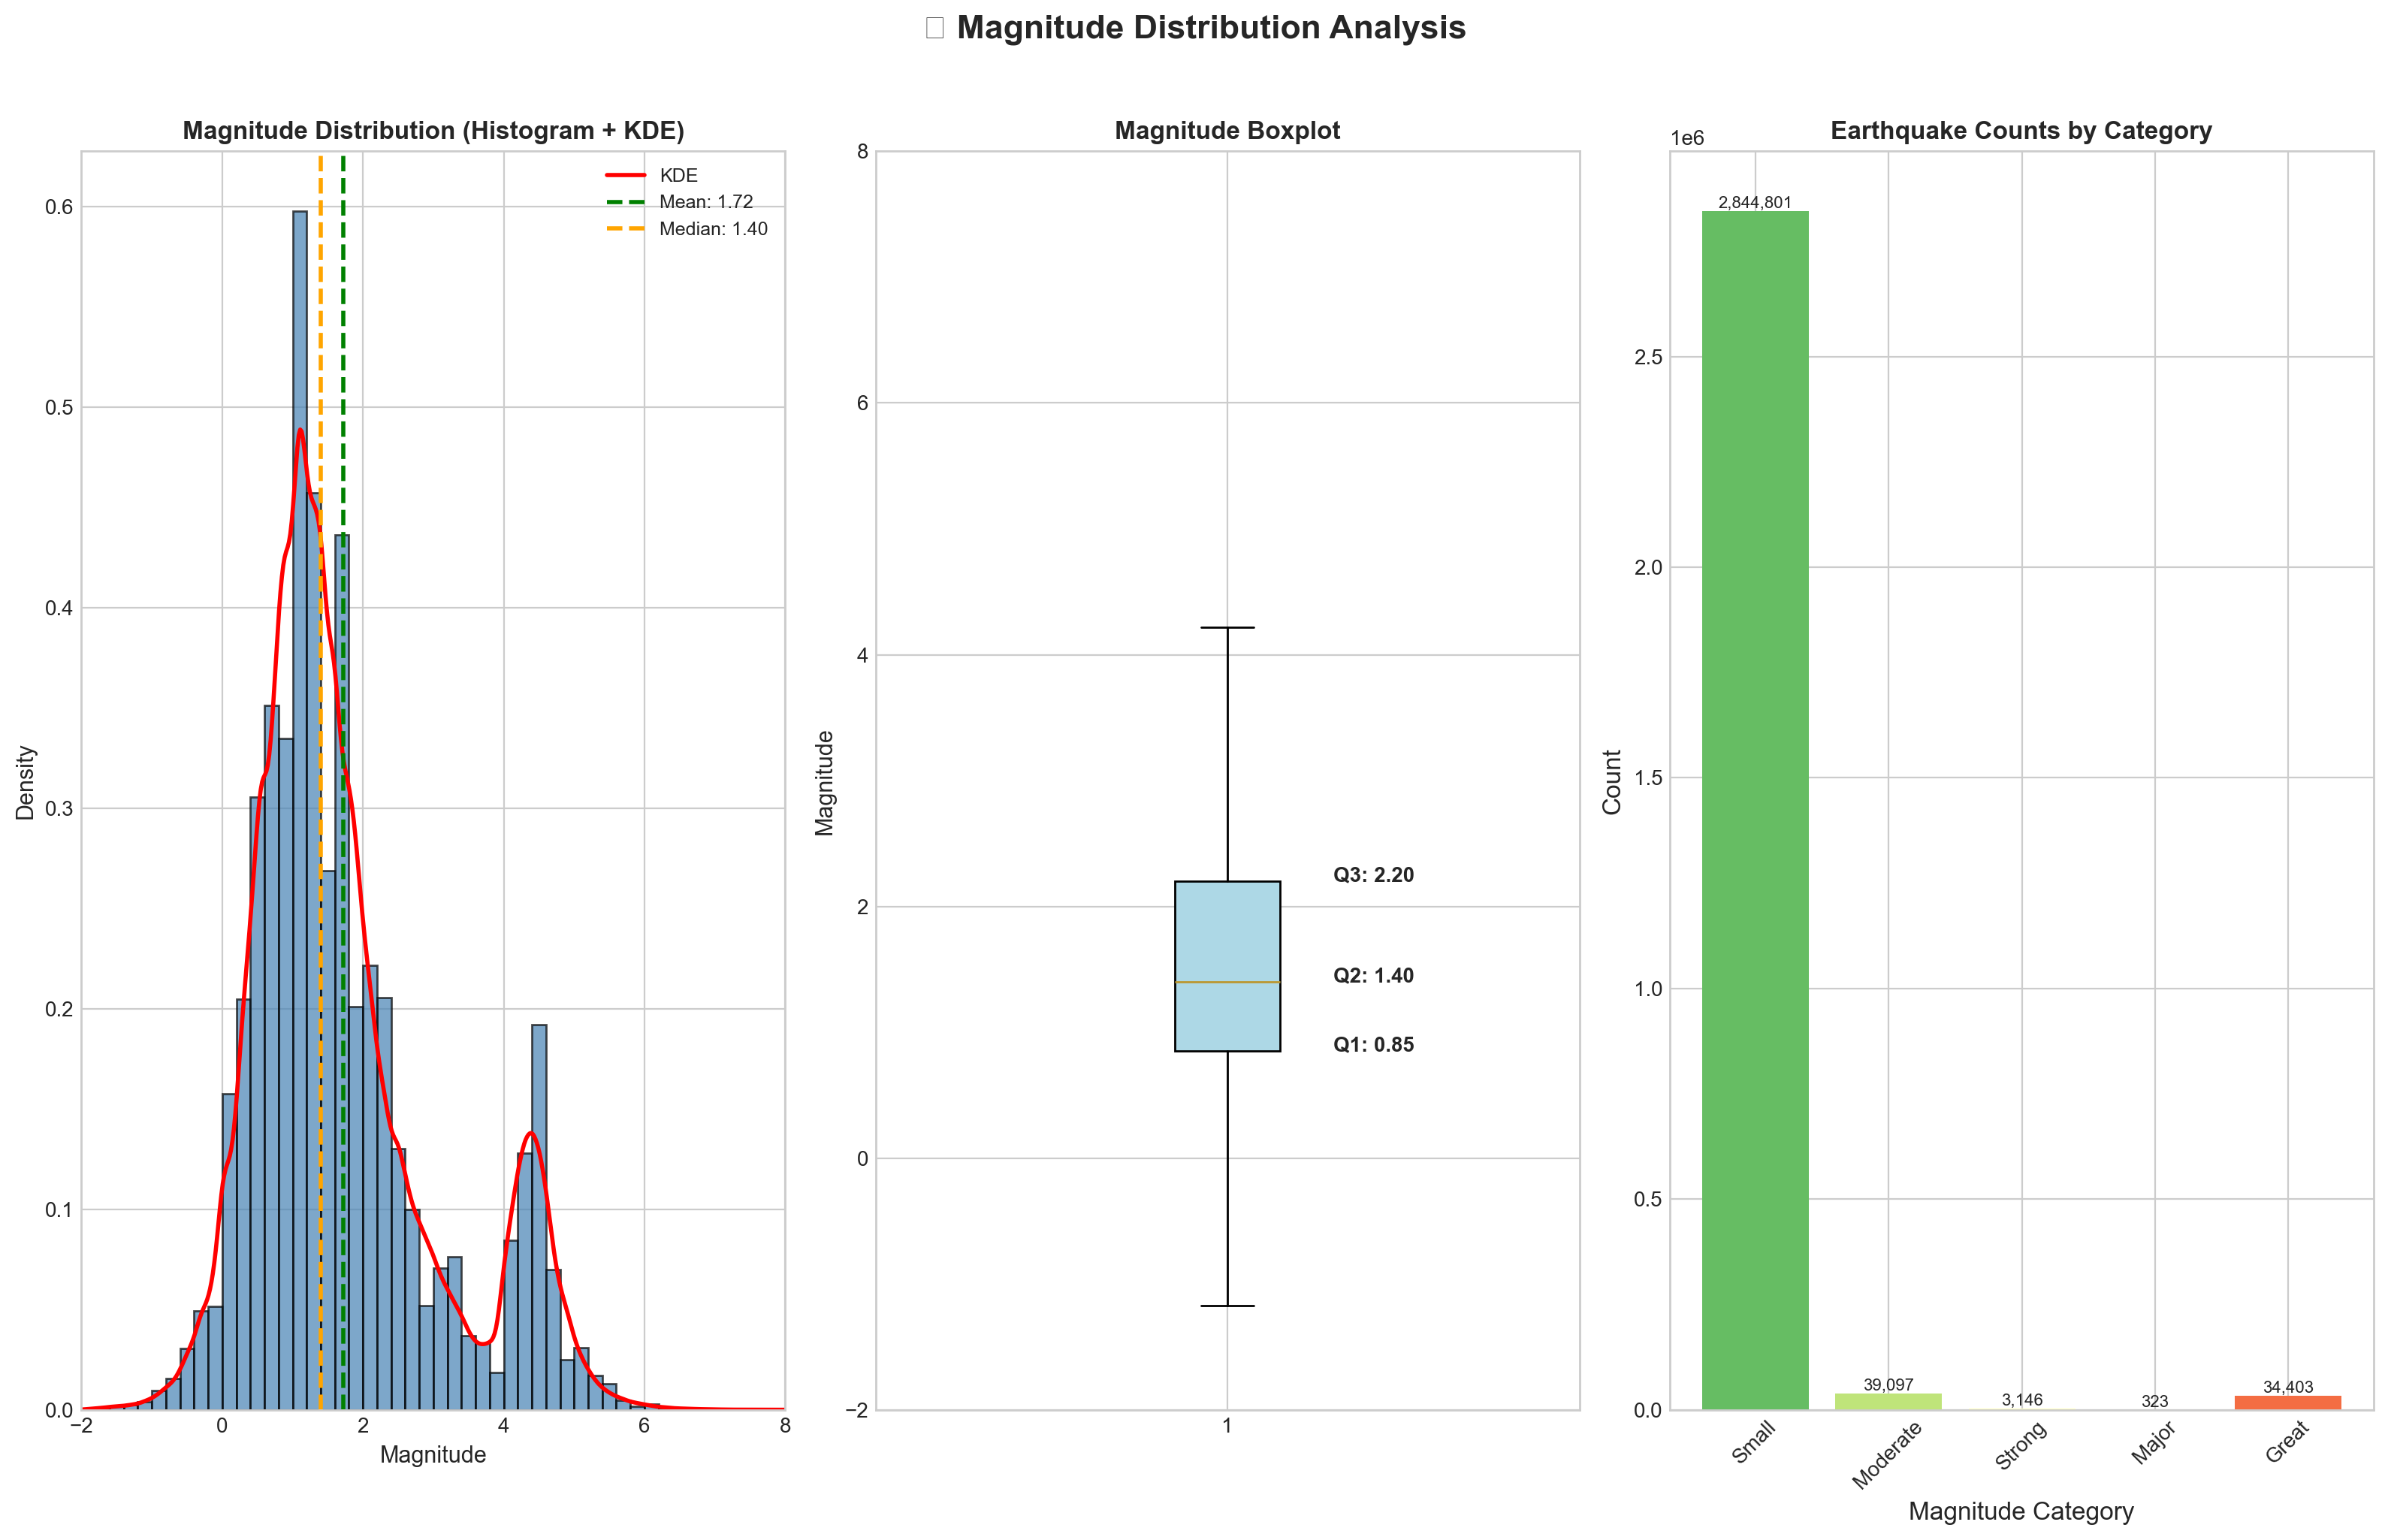
\includegraphics[width=0.95\textwidth]{figures/magnitude_distribution.png}
    \caption{Magnitude distribution analysis. Left: Histogram showing right-skewed distribution with mean=1.72 and median=1.40. Center: Boxplot with quartiles Q1=0.90, Q2=1.40, Q3=2.30. Right: Counts by magnitude category showing extreme class imbalance.}
    \label{fig:magnitude_dist}
\end{figure}

\textbf{Key statistics:}
\begin{itemize}
    \item \textbf{Mean}: 1.72, \textbf{Median}: 1.40, \textbf{Std}: 1.32
    \item \textbf{Range}: -9.99 to 9.1
    \item \textbf{Distribution}: Right-skewed (skewness = 0.85), following the Gutenberg-Richter law
\end{itemize}

\textbf{Category breakdown:}
\begin{itemize}
    \item Small (M $<$ 4.0): 2,844,801 events (\textbf{97.4\%})
    \item Moderate (4.0--5.0): 39,097 events (1.3\%)
    \item Strong (5.0--6.0): 34,403 events (1.2\%)
    \item Major (M $\geq$ 7.0): 323 events (0.01\%)
\end{itemize}

The extreme class imbalance (97.4\% small earthquakes) reflects the physics of earthquake generation---small ruptures are far more common than large ones.

\subsubsection{Depth-Magnitude Relationship}

Figure \ref{fig:depth_vs_mag} examines the relationship between earthquake depth and magnitude.

\begin{figure}[H]
    \centering
    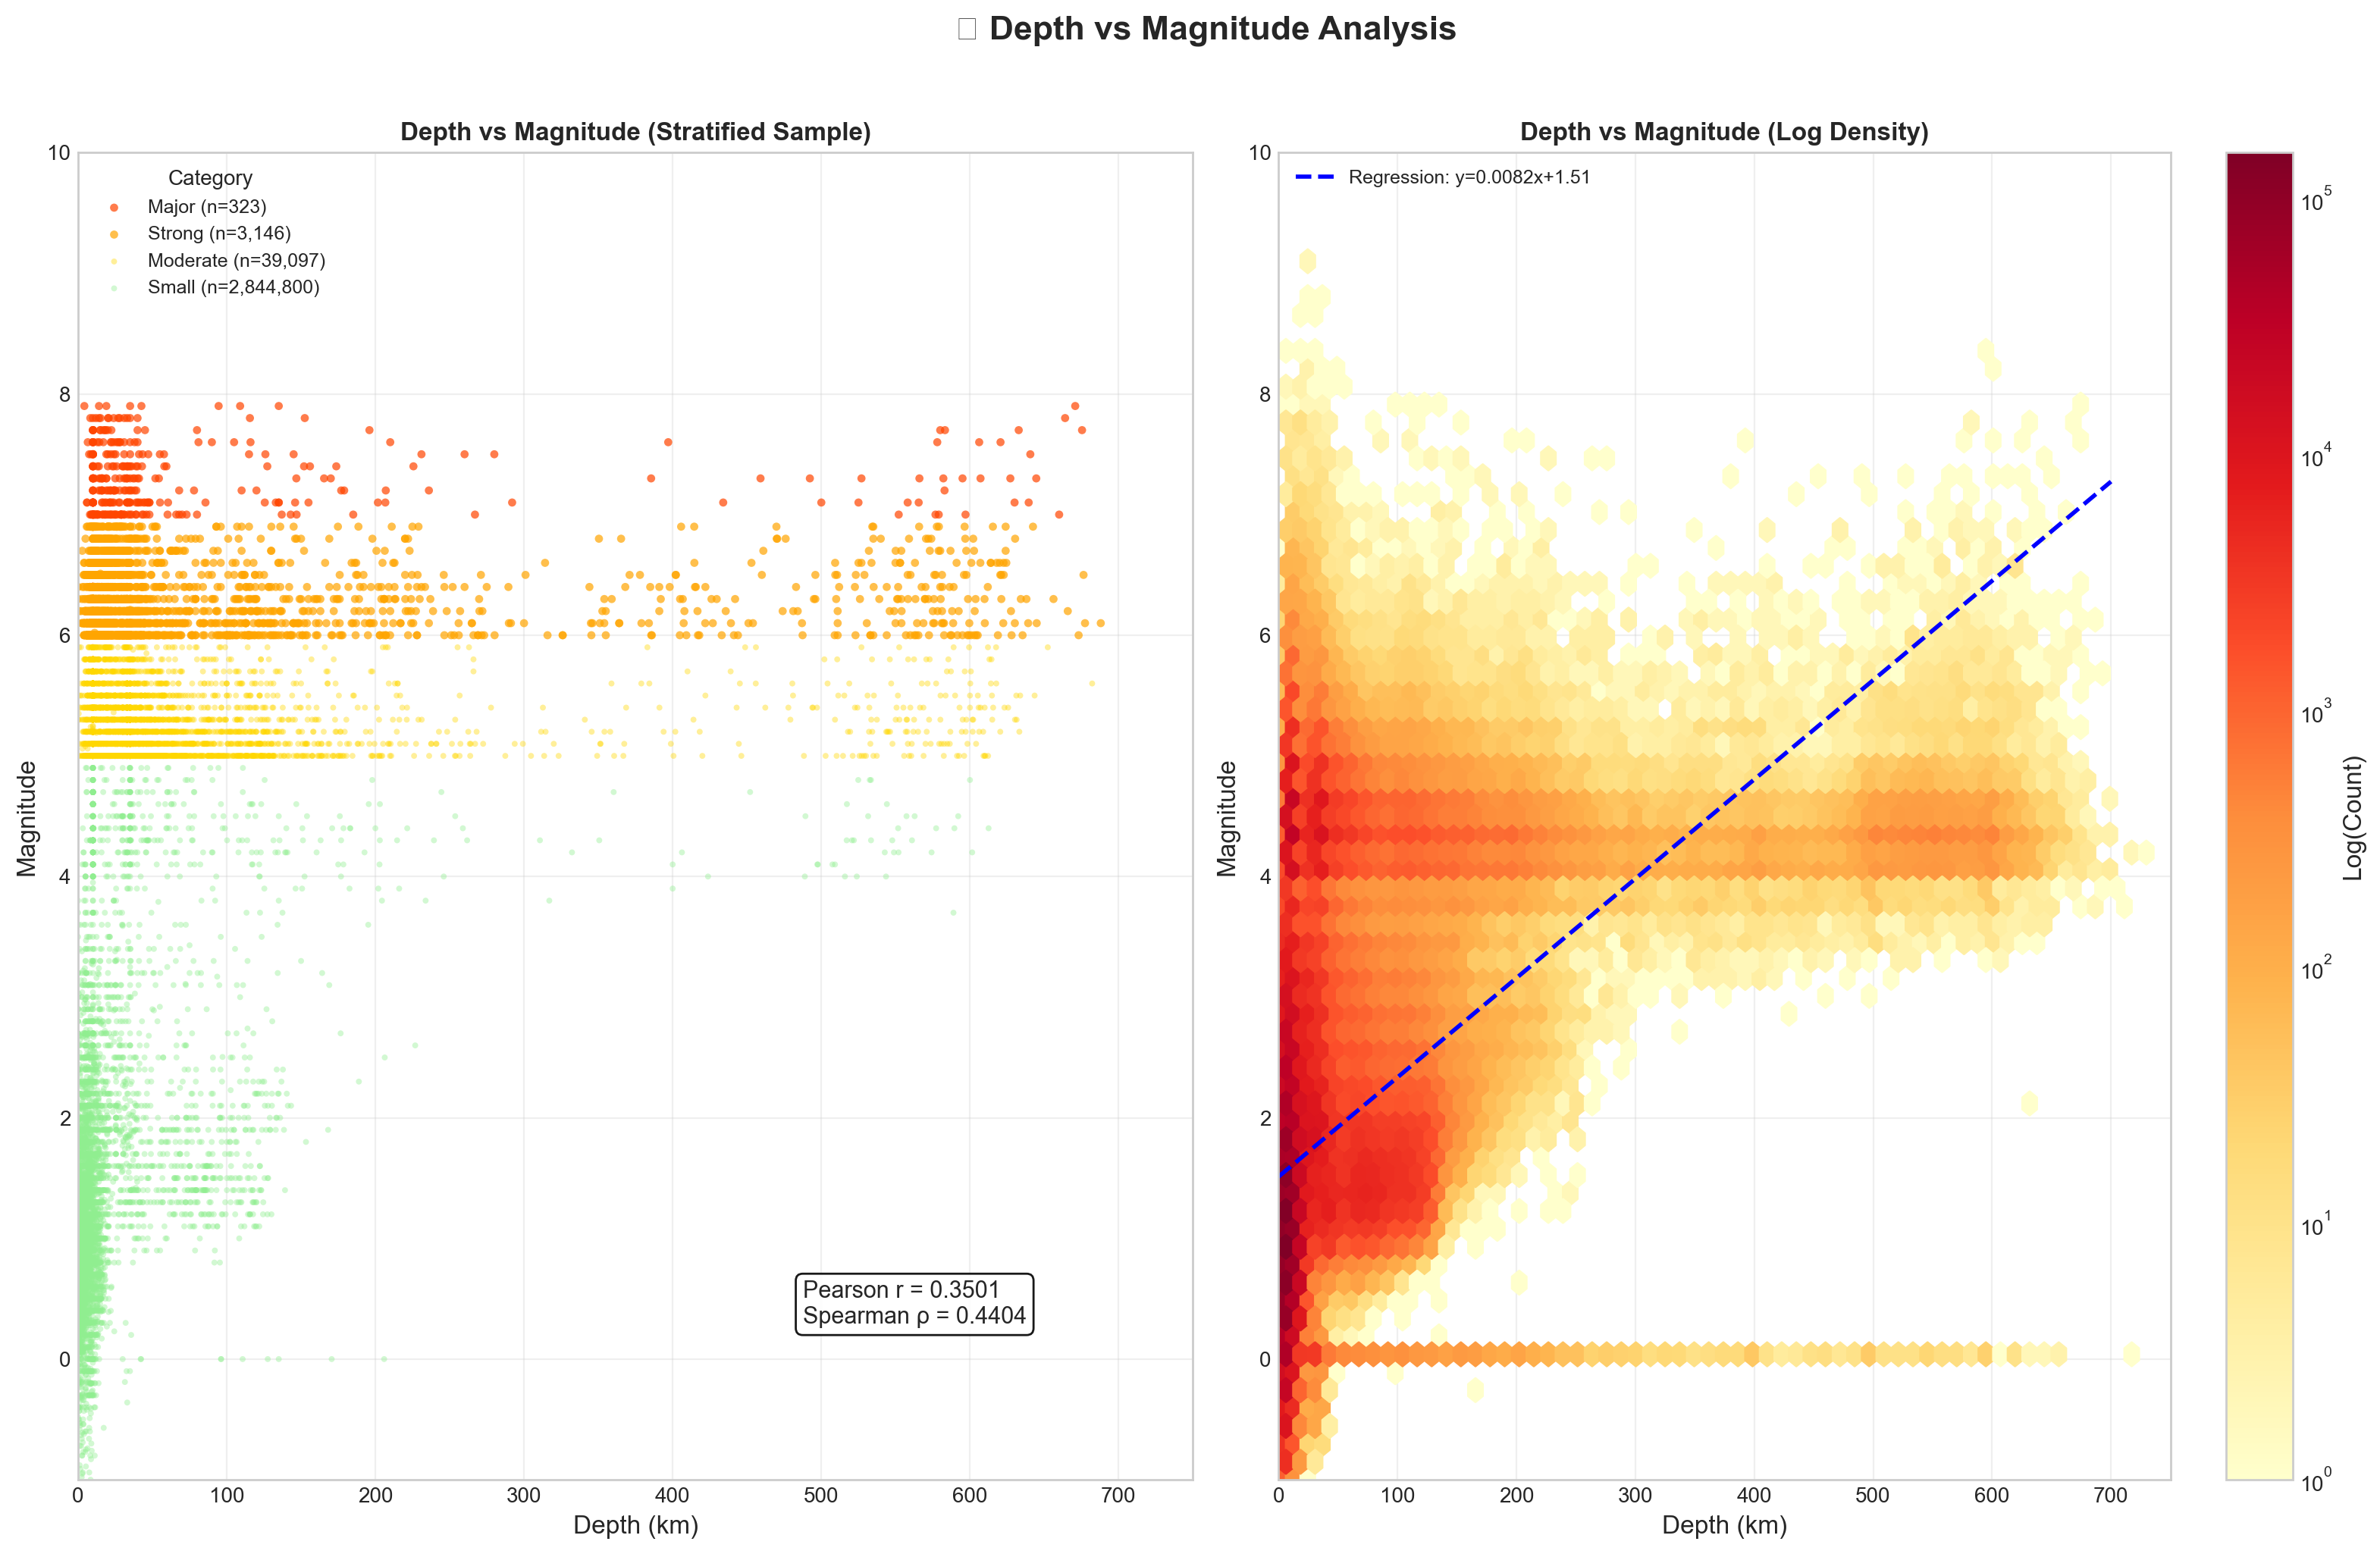
\includegraphics[width=0.95\textwidth]{figures/depth_vs_magnitude_scatter.png}
    \caption{Depth vs Magnitude relationship. Left: Stratified scatter plot showing all magnitude categories clearly with correlation statistics (Pearson r = 0.35, Spearman $\rho$ = 0.44). Right: Hexbin log-density plot showing concentration of small, shallow earthquakes with regression line.}
    \label{fig:depth_vs_mag}
\end{figure}

\textbf{Key findings:}
\begin{itemize}
    \item \textbf{Moderate positive correlation}: r = 0.35, meaning deeper earthquakes tend to have larger magnitudes on average.
    \item \textbf{Detection bias}: Small earthquakes at great depth are harder to detect---seismic waves attenuate before reaching surface seismometers.
    \item \textbf{Shallow earthquakes span all magnitudes}: From micro-earthquakes (M $<$ 0) to great earthquakes (M $>$ 8).
\end{itemize}

\subsubsection{Energy-Magnitude Relationship}

Figure \ref{fig:mag_energy} demonstrates why magnitude prediction is critical---energy scales exponentially.

\begin{figure}[H]
    \centering
    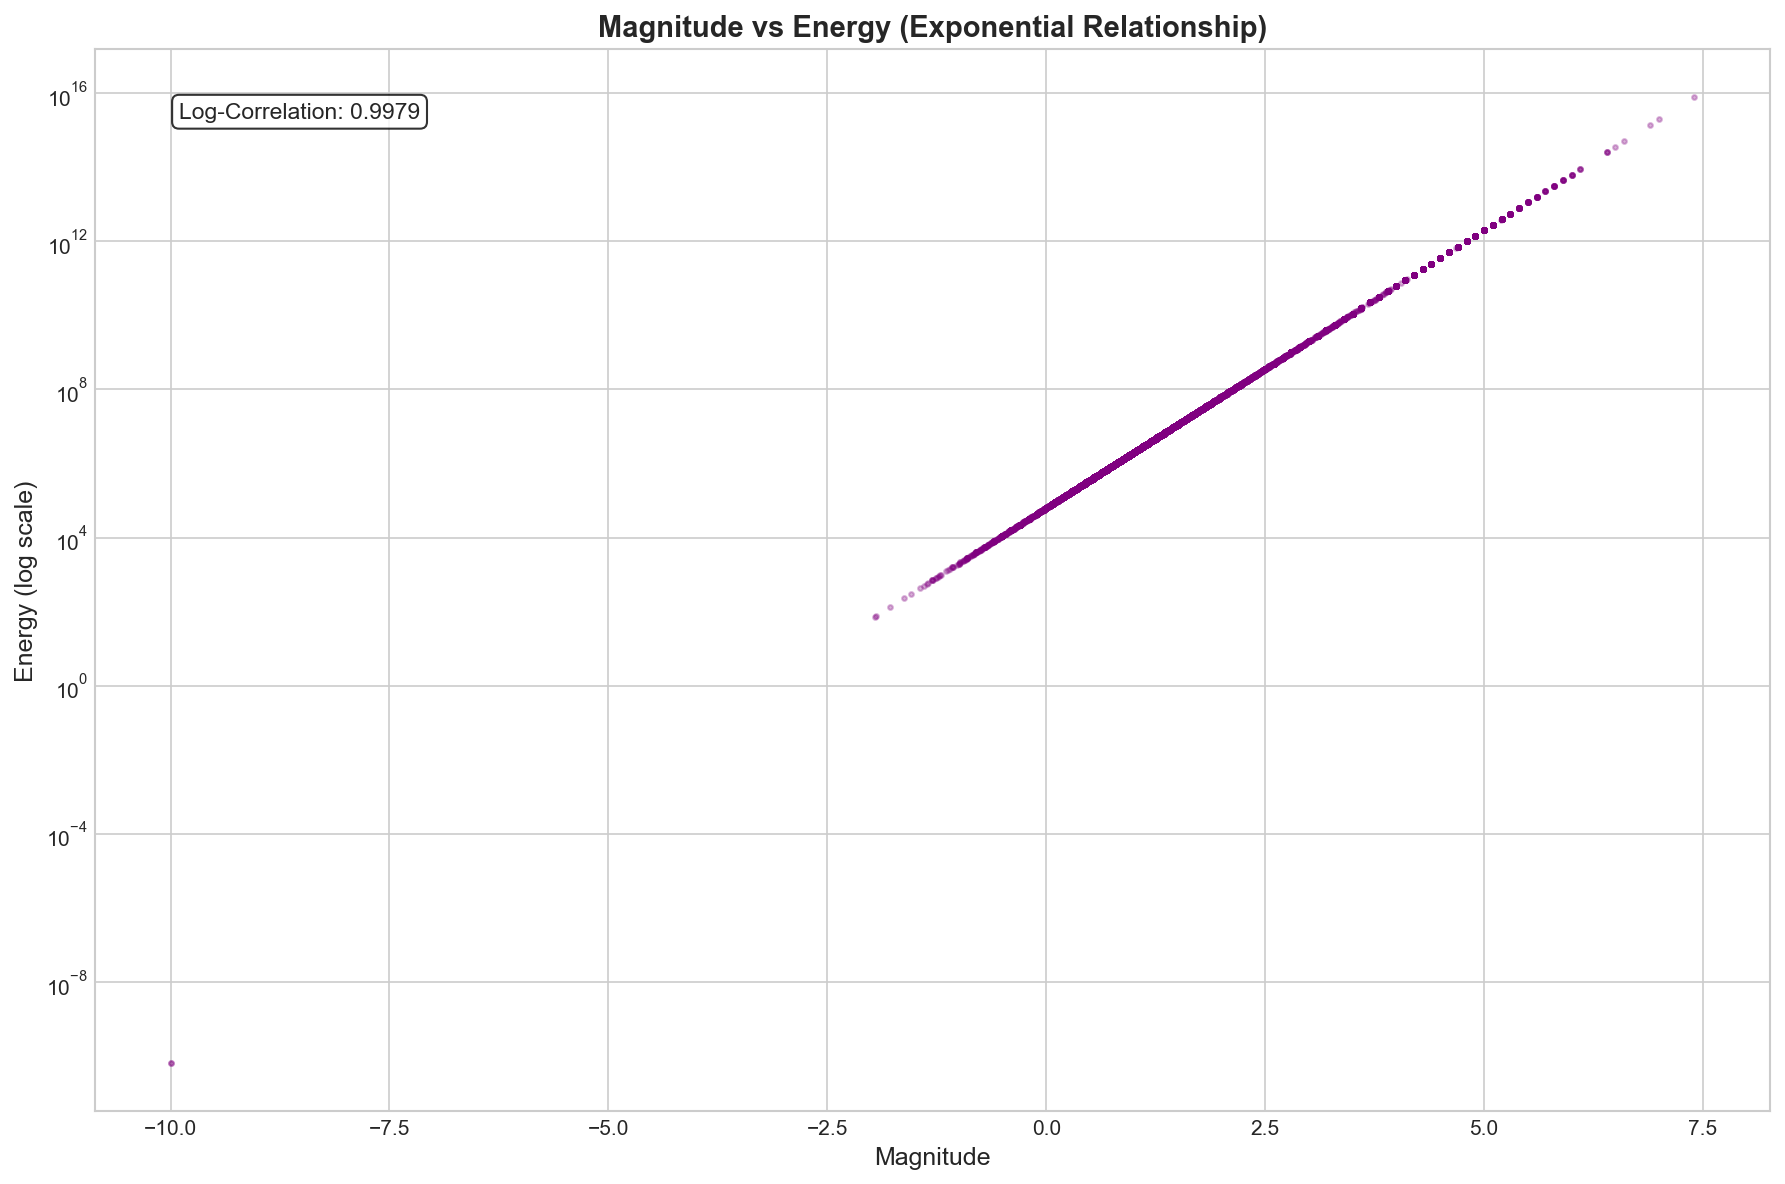
\includegraphics[width=0.75\textwidth]{figures/magnitude_vs_energy.png}
    \caption{Magnitude vs Energy on semi-log scale. Linear trend confirms exponential relationship: each magnitude unit releases approximately 31.6 times more energy.}
    \label{fig:mag_energy}
\end{figure}

The energy-magnitude relationship follows:
\begin{equation}
\log_{10}(E) = 1.5M + 4.8 \text{ (Joules)}
\end{equation}

This means a M 9.0 earthquake releases \textbf{1 million times} more energy than a M 5.0, explaining why great earthquakes cause catastrophic damage.

%==============================================================================
\subsection{Depth Analysis}
%==============================================================================

\subsubsection{Depth Distribution}

Figure \ref{fig:depth_dist} shows the distribution of earthquake depths, revealing the vertical structure of seismic activity.

\begin{figure}[H]
    \centering
    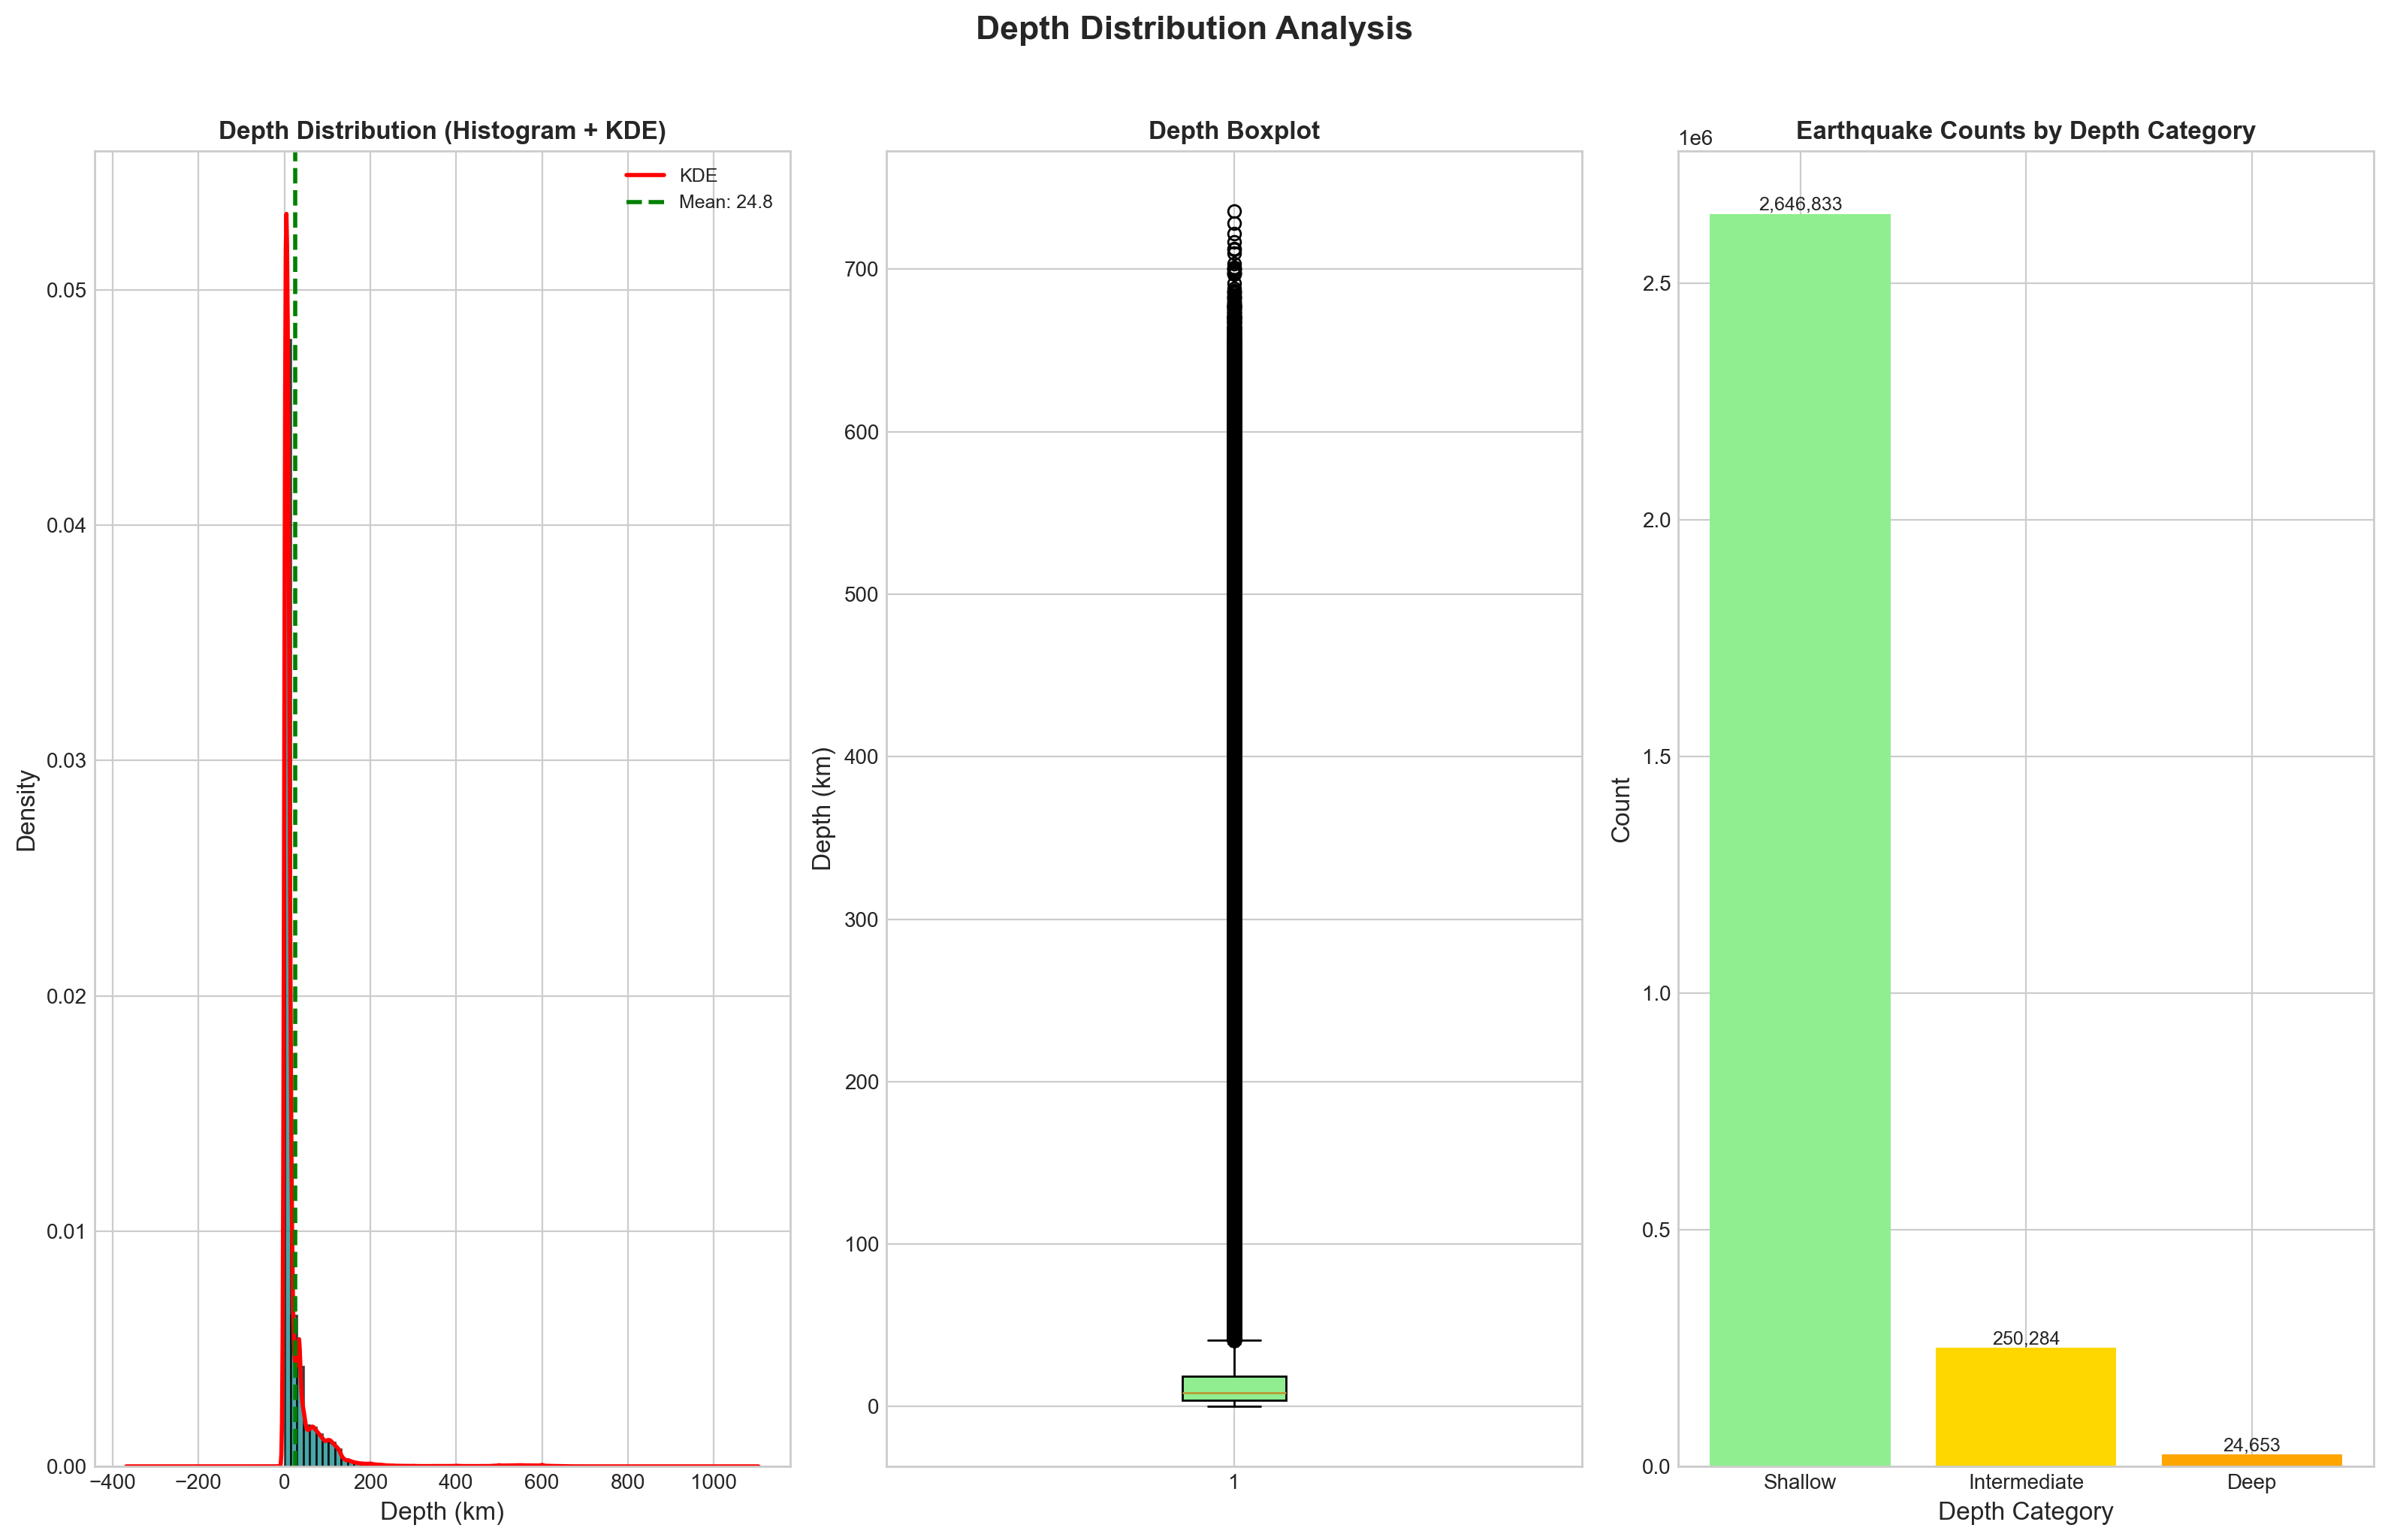
\includegraphics[width=0.95\textwidth]{figures/depth_distribution.png}
    \caption{Depth distribution analysis. Left: Histogram showing concentration at shallow depths (mean=24.8 km, median=8.6 km). Center: Boxplot showing outliers up to 735.8 km. Right: Category breakdown showing Shallow earthquakes dominate at 90.6\%.}
    \label{fig:depth_dist}
\end{figure}

\textbf{Depth statistics:}
\begin{itemize}
    \item \textbf{Mean}: 24.8 km, \textbf{Median}: 8.6 km
    \item \textbf{Maximum}: 735.8 km (near the physical limit for earthquakes)
\end{itemize}

\textbf{Category distribution:}
\begin{itemize}
    \item \textbf{Shallow} ($<$ 70 km): 2,646,833 events (\textbf{90.6\%}) --- Most destructive due to proximity to surface
    \item \textbf{Intermediate} (70--300 km): 231,458 events (7.9\%) --- Associated with subduction zones
    \item \textbf{Deep} ($>$ 300 km): 43,477 events (1.5\%) --- Only in active subduction zones (Tonga-Kermadec, South America)
\end{itemize}

\subsubsection{Geographic Patterns of Depth}

Deep earthquakes occur only in specific tectonic settings:
\begin{itemize}
    \item \textbf{Shallow earthquakes}: Occur everywhere with tectonic activity
    \item \textbf{Intermediate depth}: Concentrated in subduction zones (Japan, South America, Indonesia)
    \item \textbf{Deep earthquakes}: Only where cold oceanic lithosphere descends into the mantle
\end{itemize}

This geographic constraint means \textbf{latitude and longitude are informative features} for depth classification---certain regions simply do not produce deep earthquakes.

%==============================================================================
\subsection{Geospatial Analysis}
%==============================================================================

\subsubsection{Global Earthquake Distribution}

Figure \ref{fig:locations} shows the spatial distribution of earthquakes, revealing natural clustering patterns along tectonic plate boundaries.

\begin{figure}[H]
    \centering
    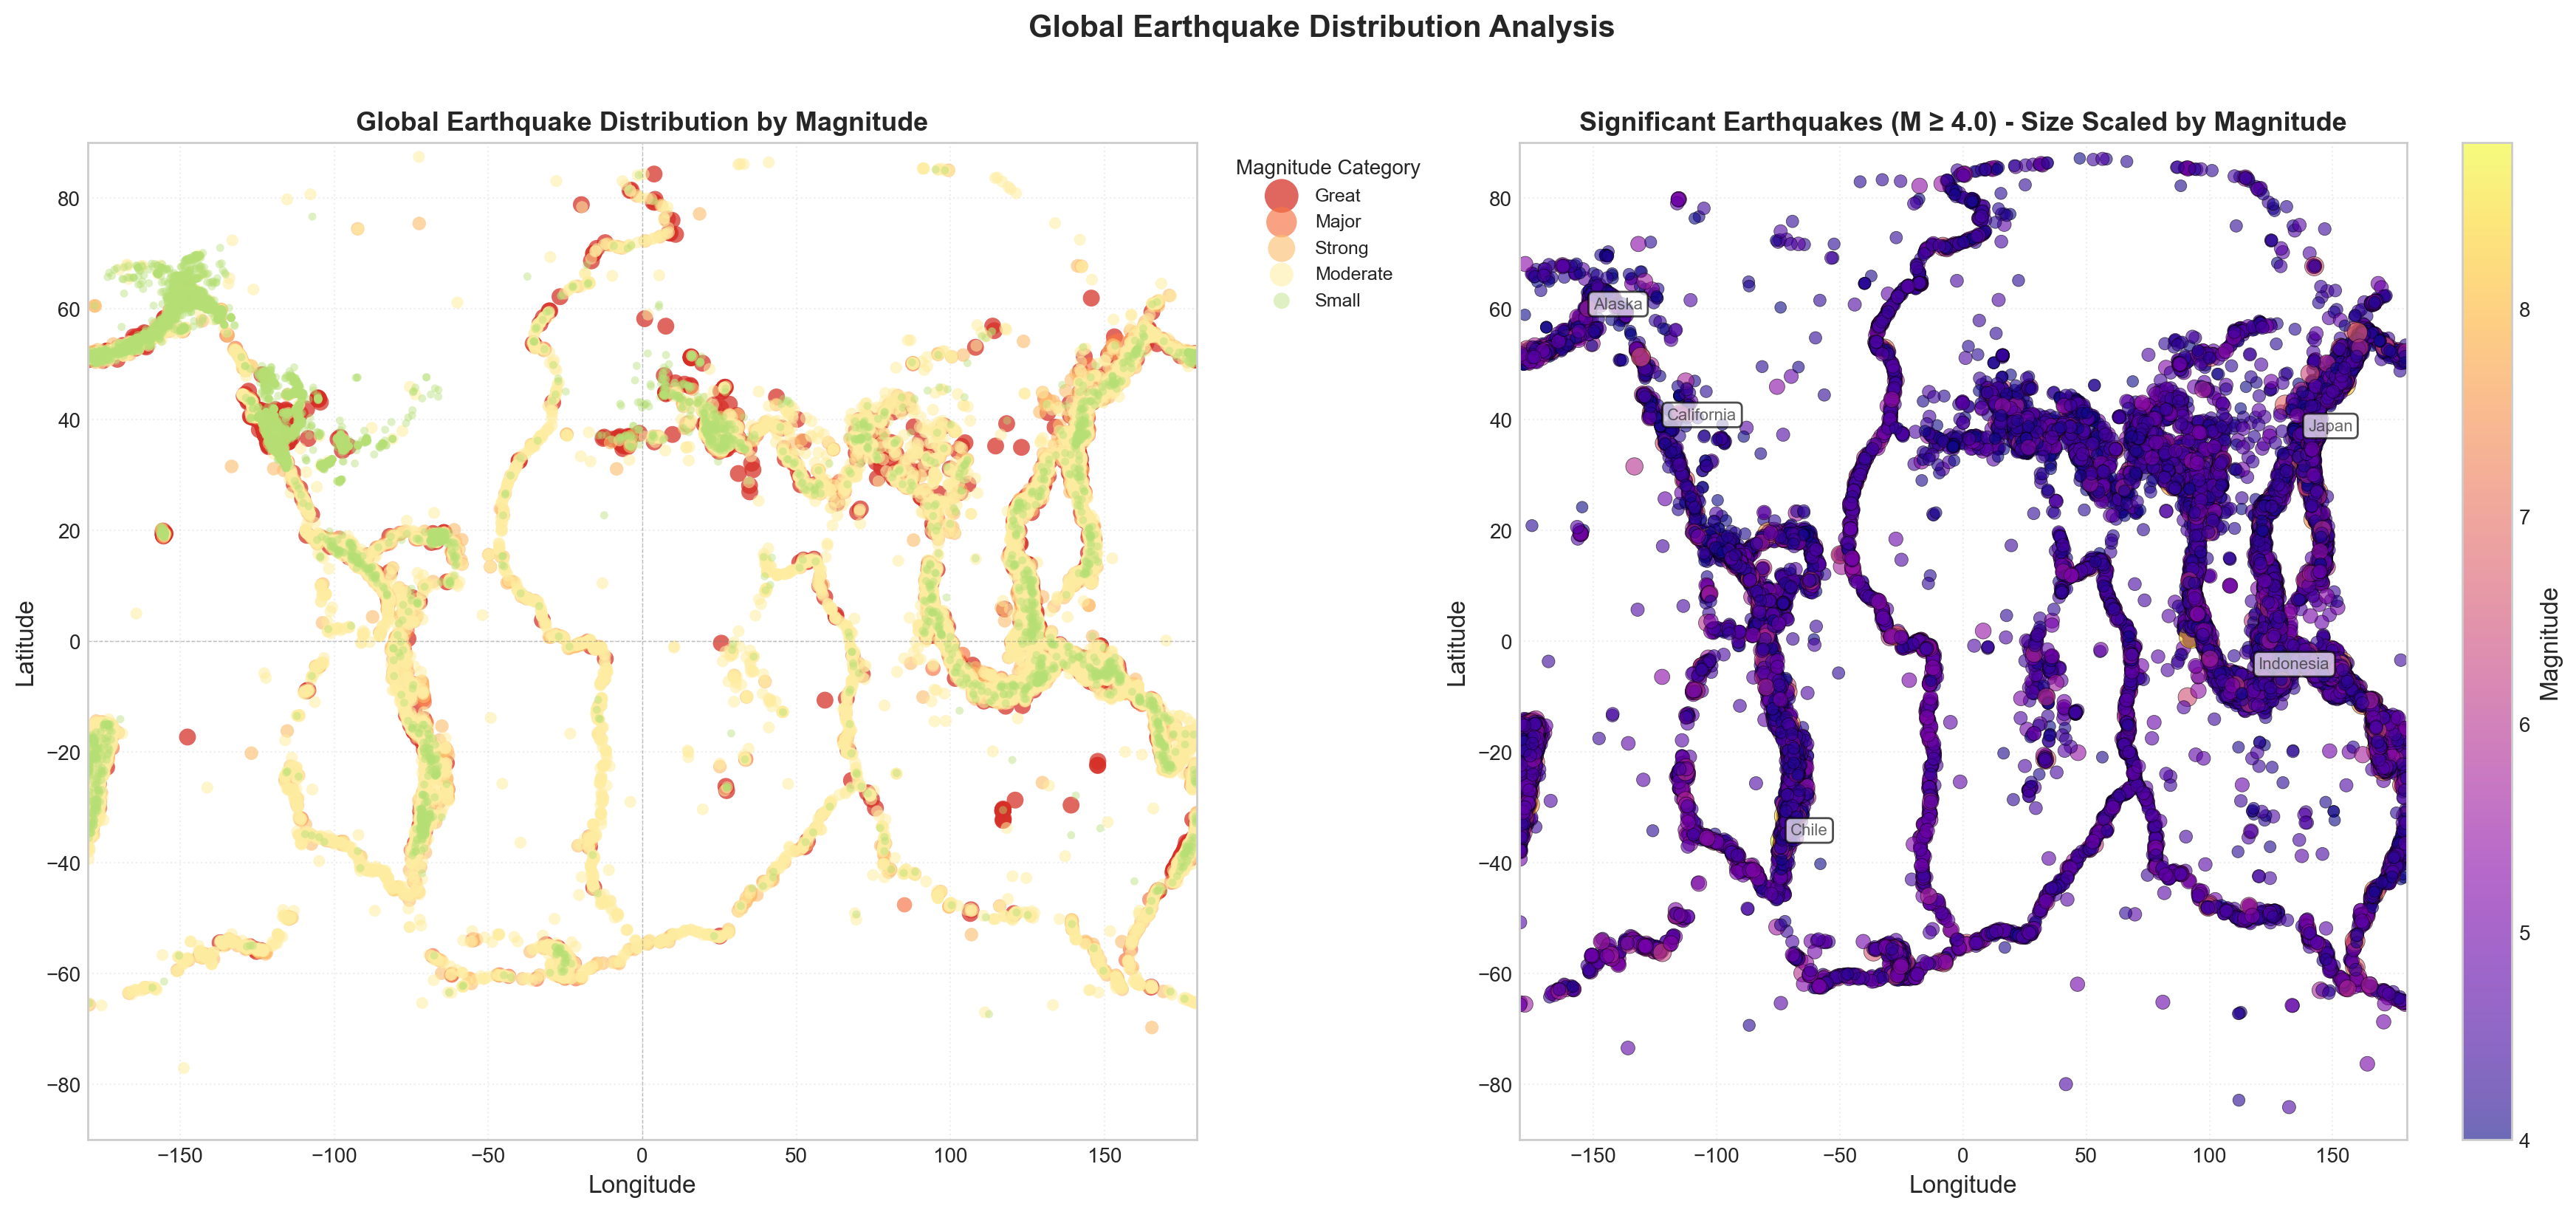
\includegraphics[width=0.95\textwidth]{figures/earthquake_locations.png}
    \caption{Global earthquake distribution. Left: All earthquakes colored by magnitude category showing concentration along plate boundaries. Right: Significant earthquakes (M $\geq$ 4.0) with annotated seismic zones. The Pacific Ring of Fire is clearly visible.}
    \label{fig:locations}
\end{figure}

\textbf{Major seismic zones identified:}
\begin{itemize}
    \item \textbf{Pacific Ring of Fire}: Accounts for $\sim$80\% of significant earthquakes, encircling the Pacific Ocean
    \item \textbf{California/San Andreas}: Dense cluster along transform fault
    \item \textbf{Alaska-Aleutian}: High-frequency cluster at subduction zone
    \item \textbf{Japan-Kamchatka}: Major subduction zone cluster
    \item \textbf{Indonesia}: Sunda arc subduction cluster
    \item \textbf{Chile/South America}: Nazca plate subduction cluster
\end{itemize}

\subsubsection{Earthquake Density Heatmap}

Figure \ref{fig:density} provides density visualization essential for identifying seismic hotspots.

\begin{figure}[H]
    \centering
    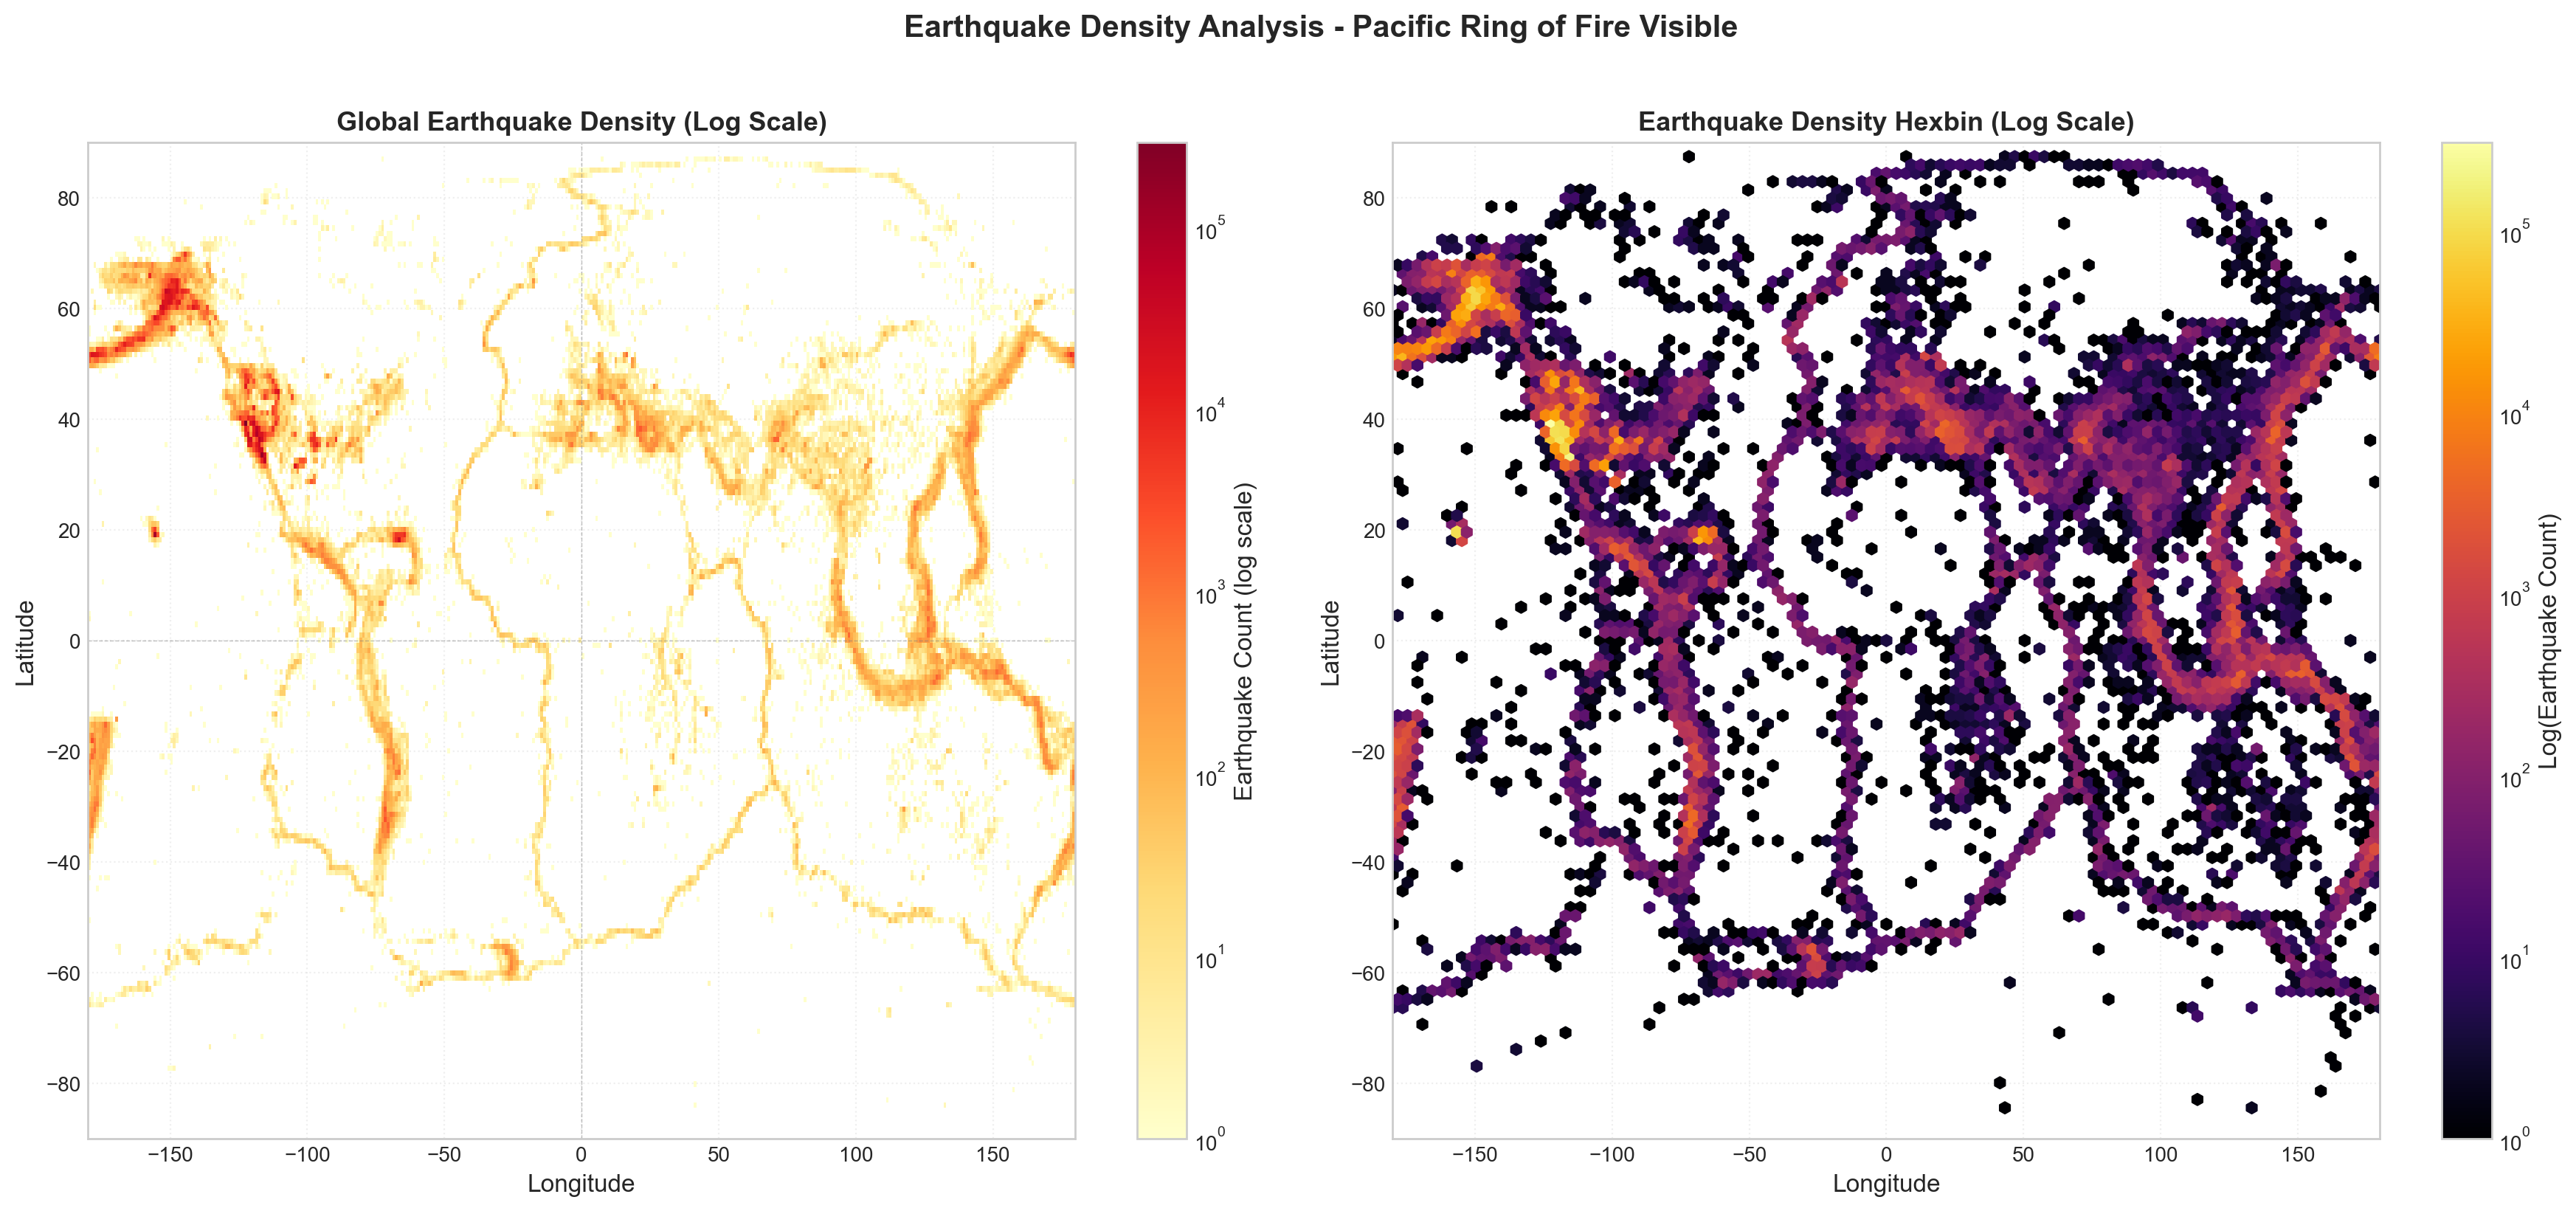
\includegraphics[width=0.95\textwidth]{figures/earthquake_density.png}
    \caption{Earthquake density heatmap with logarithmic color scale. Left: 2D histogram (1-degree resolution). Right: Hexbin smoothed visualization. High-density regions represent seismic hotspots along plate boundaries.}
    \label{fig:density}
\end{figure}

The density map validates tectonic theory---seismicity follows plate boundaries with remarkable precision. The Pacific Ring of Fire clearly emerges as the dominant seismic belt.

\subsubsection{Regional Statistics}

Figure \ref{fig:regional} quantifies earthquake frequency and intensity by region.

\begin{figure}[H]
    \centering
    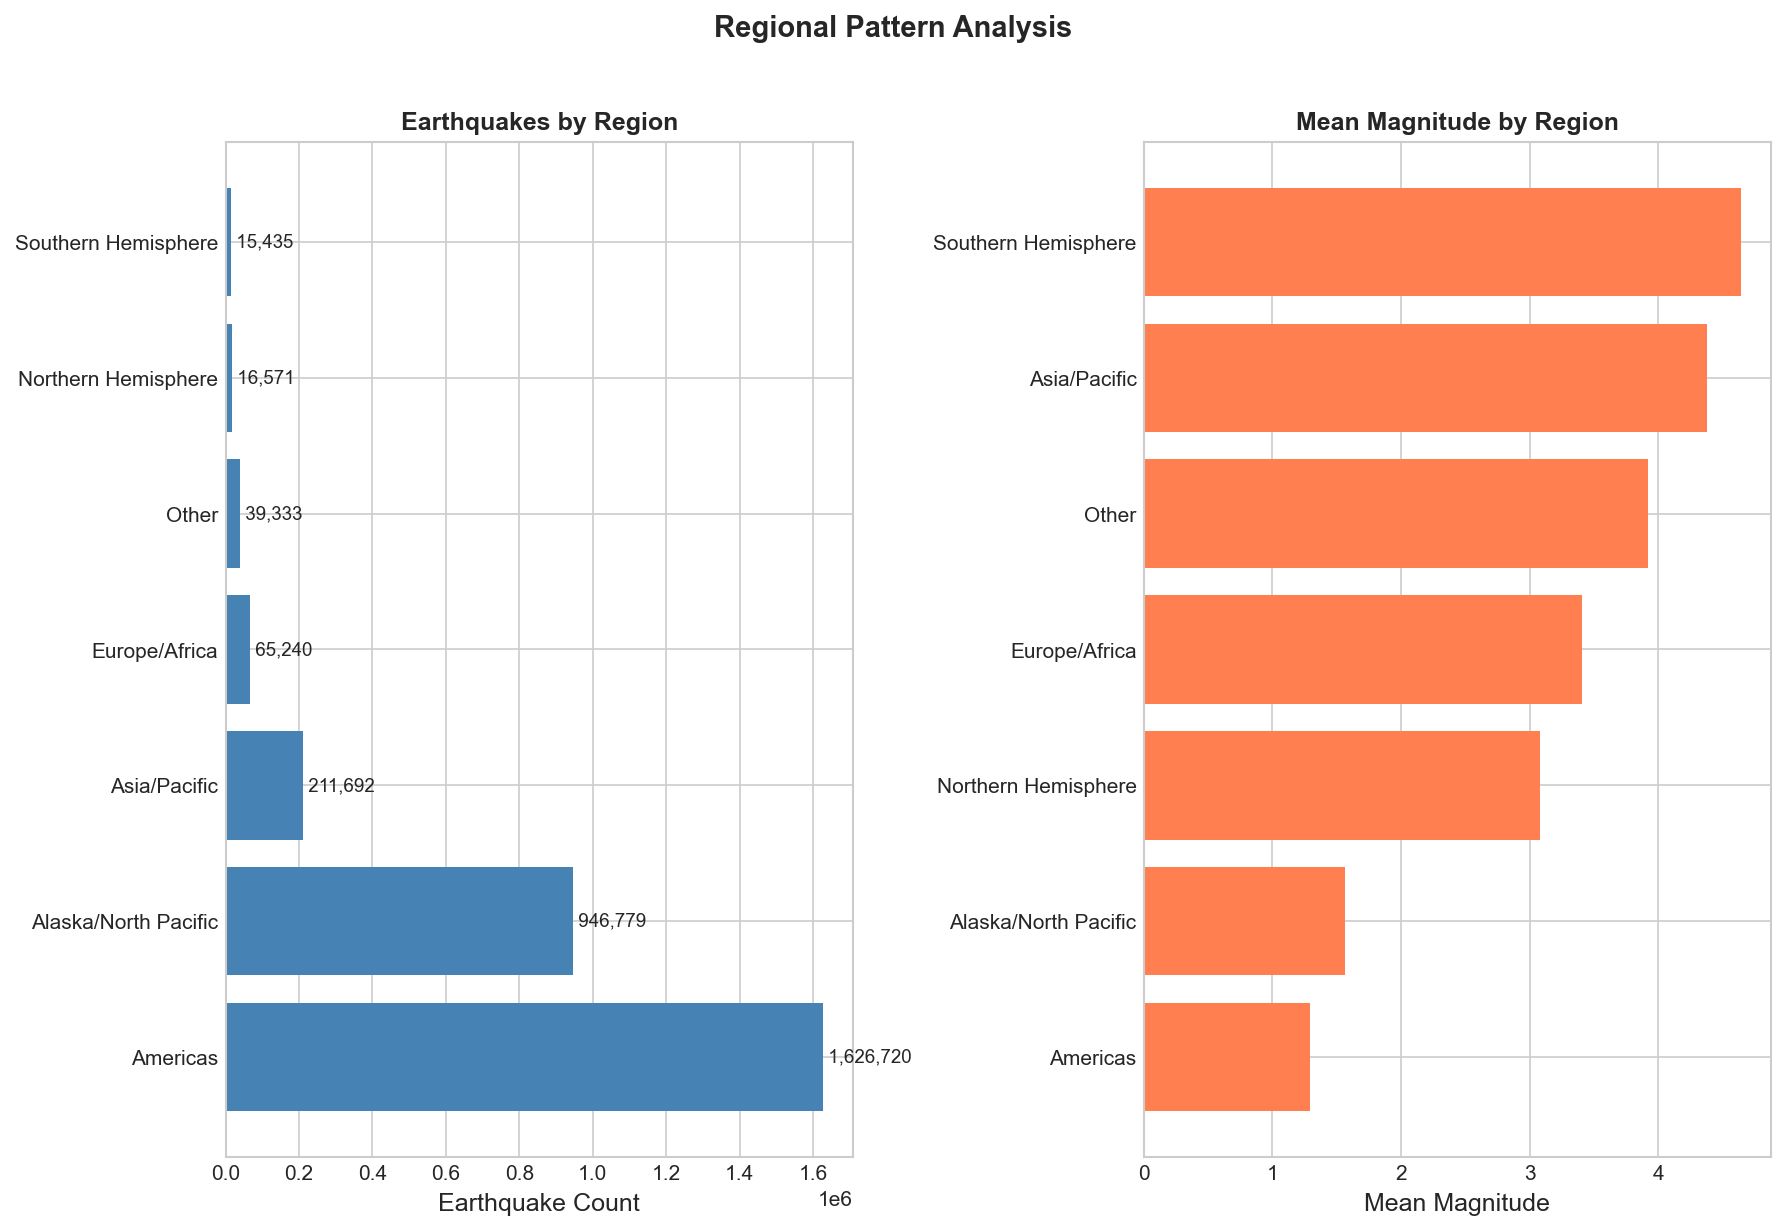
\includegraphics[width=0.85\textwidth]{figures/regional_patterns.png}
    \caption{Regional earthquake patterns. Left: Event counts showing Americas with highest count (1.6M events). Right: Mean magnitude by region showing Asia/Pacific with highest average (4.38).}
    \label{fig:regional}
\end{figure}

\textbf{Regional findings:}
\begin{itemize}
    \item \textbf{Americas}: 1,595,101 events, mean magnitude 1.47 --- Highest count due to dense monitoring
    \item \textbf{Alaska/North Pacific}: 946,527 events, mean magnitude 1.85
    \item \textbf{Asia/Pacific}: 210,166 events, mean magnitude \textbf{4.38} --- Fewer events but much larger on average
    \item \textbf{Detection bias}: Regions with dense networks detect more small earthquakes; less-monitored regions only record larger events
\end{itemize}

%==============================================================================
\subsection{Temporal Trends}
%==============================================================================

Figure \ref{fig:temporal} examines earthquake patterns over time.

\begin{figure}[H]
    \centering
    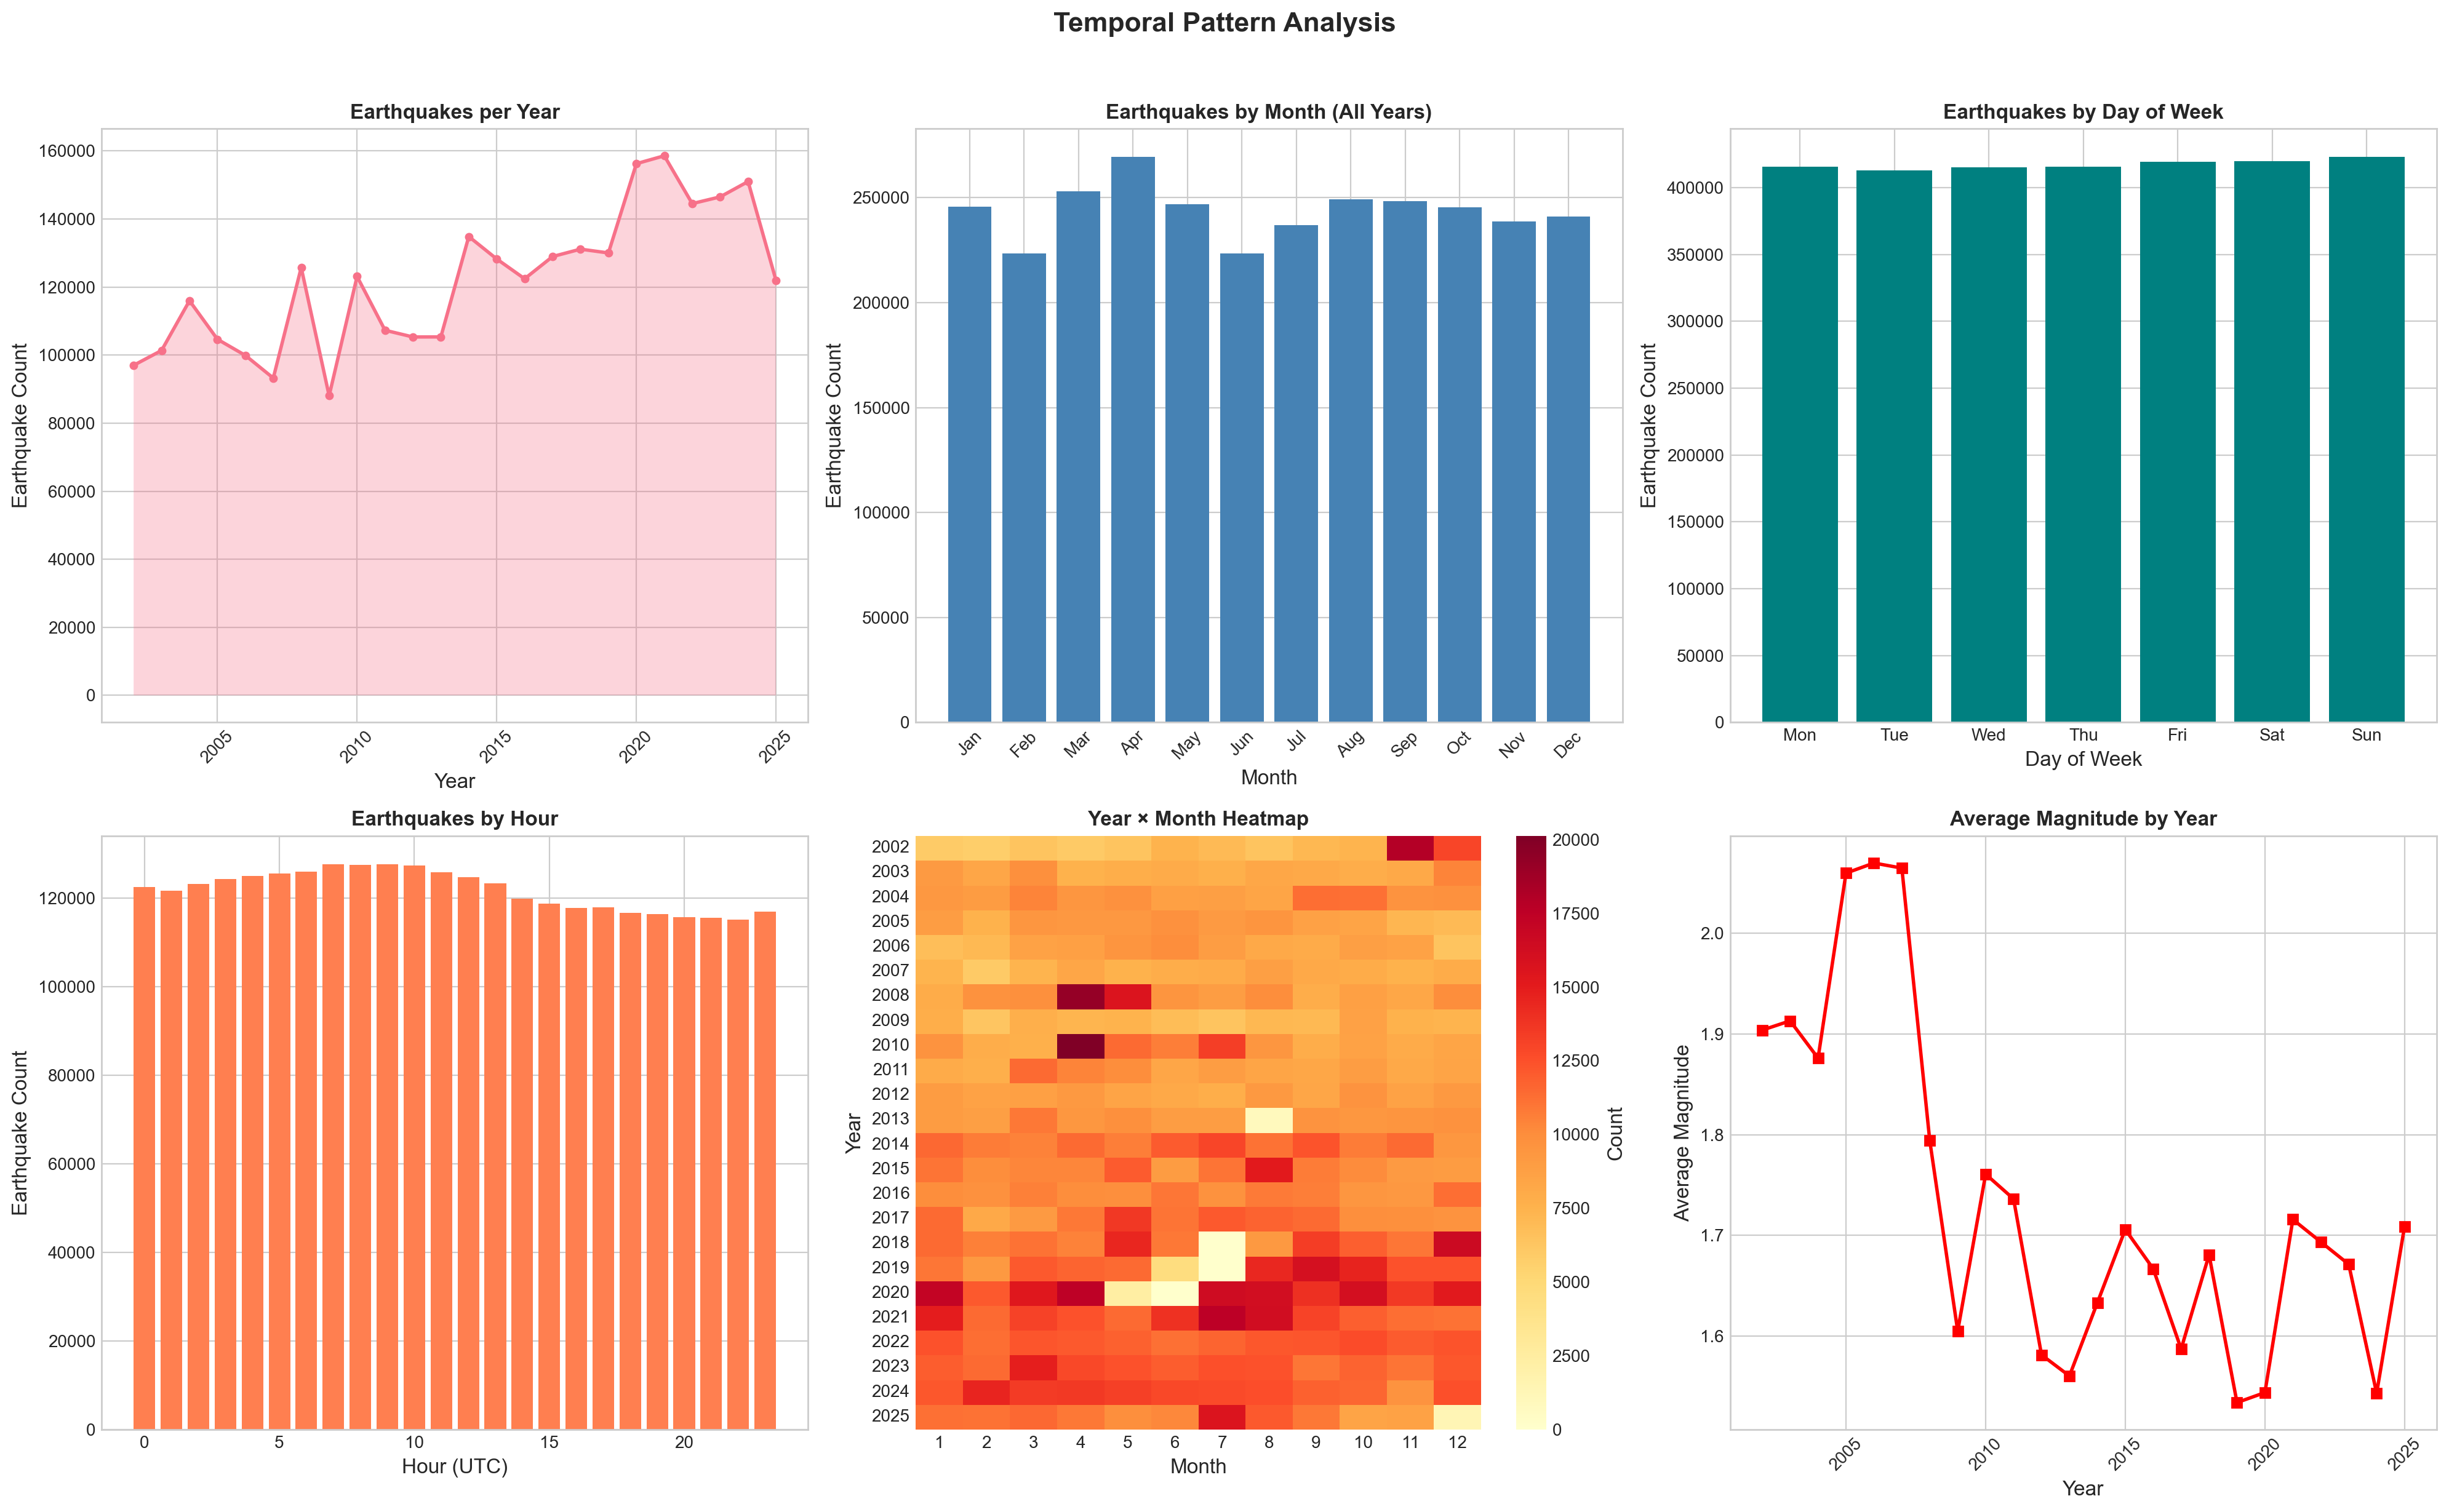
\includegraphics[width=0.95\textwidth]{figures/temporal_patterns.png}
    \caption{Temporal pattern analysis. Top-left: Yearly counts showing apparent increase from 2002--2025. Bottom-right: Average magnitude remaining stable around 1.7.}
    \label{fig:temporal}
\end{figure}

\textbf{Key insight}: The apparent increase in earthquake counts over time does \textbf{not} indicate more earthquakes are occurring. Evidence:
\begin{itemize}
    \item Average magnitude has remained stable around 1.7
    \item The increase is entirely in small earthquakes
    \item Cause: Expansion of seismic monitoring networks and improved detection
\end{itemize}

%==============================================================================
\subsection{Key Findings Summary}
%==============================================================================

\begin{table}[H]
\centering
\begin{tabular}{|p{4cm}|p{9cm}|}
\hline
\textbf{Finding} & \textbf{Implication} \\
\hline
97.4\% small earthquakes (M $<$ 4) & Severe class imbalance; need weighted sampling or loss functions \\
\hline
90.6\% shallow earthquakes & Depth classification heavily imbalanced toward Shallow class \\
\hline
Depth-Magnitude correlation r=0.35 & Depth is a useful predictive feature for magnitude \\
\hline
Pacific Ring of Fire = 80\% of large earthquakes & Strong spatial clustering; geographic features highly informative \\
\hline
Deep earthquakes only in subduction zones & Location (lat/lon) can predict depth category \\
\hline
Detection bias in counts & More monitoring $\rightarrow$ more small earthquakes detected \\
\hline
\end{tabular}
\caption{Summary of EDA findings and modeling implications}
\end{table}

\textbf{Data challenges to address:}
\begin{itemize}
    \item \textbf{Class imbalance}: Both magnitude and depth distributions are heavily skewed
    \item \textbf{Detection bias}: Station count (nst) correlates with magnitude but may not be causal
    \item \textbf{Geographic bias}: Dense monitoring in Americas skews toward detecting small earthquakes
\end{itemize}
